\documentclass[10pt]{article}   	 
\usepackage{geometry}                		 
\geometry{a4paper}  
 
%\usepackage{draftwatermark}
%\SetWatermarkAngle{45}
%\SetWatermarkLightness{0.8}
%\SetWatermarkFontSize{4cm}
%\SetWatermarkScale{2}
%\SetWatermarkText{DRAFT  - NO DISTRIBUTION }
               		
\usepackage{graphicx}		
\usepackage{hyperref}		
\usepackage{amssymb}
\usepackage{longtable}
\usepackage{listings} \lstset{numbers=left, numberstyle=\tiny, numbersep=5pt} \lstset{language=C}
\newcommand{\zwave}{Z-Wave \raise0.8ex\hbox{\tiny TM} }
\title{RaZberry User and Developers Documentation}
\author{z-wave.me}
\date{}							 

\begin{document}
\maketitle
\tableofcontents


\section{The RaZberry architecture}

RaZberry consists of a hardware portion  - the RaZberry  daughter board including some firmware - 
and  a portion of software that runs on the Raspberry Pi operating system. This portion of the 
software is refered to as {\bf Z-Way}.
Z-Way implements the whole Z-Wave protocol stack and offers an Application Programming Interface to implement 
third party user interfaces. Z-Way also offers some demo user interfaces to explain and prototype the solution.

\section{The RaZberry hardware}

A RaZberry hardware solution is a combination of the Raspberry PI motherboard and the RaZberry Z-Wave 
transceiver daughter board. The daughter board is connected to the motherboard using the General
IO Pin header connector of Raspberry PI. This GPIO interface offers Serial TX and RX signals, 
ground and 3.3 V VCC to power the Z-Wave transceiver board. Figure \ref{razberryboard} shows the details of the hardware.

\begin{figure} 
\begin{center}
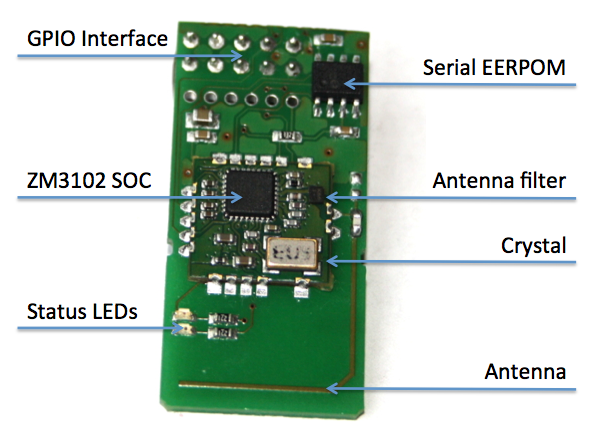
\includegraphics[scale=0.5]{pics/board.png}
\caption{RaZberry hardware}
\label{razberryboard} 
\end{center} 
\end{figure}


The daughter board consists of several components:
\begin{itemize}
\item The ZM3102 Z-Wave transceiver from Sigma Designs. This module combines a "System on 
Chip" (SOC) with a 8051 micro controller, the Z-Wave transceiver and some IO interfaces the systems 
crystal and the SAW antenna filter to comply to the national regulations
for the frequency band used:
\begin{itemize}
\item EU: 868.4 MHz (EN 300 220)
\item RU: 869.0 MHz (GKRCh/EN 300 200)
\item US: 908.4 MHz (FCC CFR47 P 15.249) 
\end{itemize}
\item The 32KB Serial EERPOM that stores the network data
\item PCBA-Antenna
\item two status LEDs: The red LED shines during inclusion and exclusion mode, the green LED is blinking on successful wireless data transmission
\end{itemize}

The micro controller of the SOC contains control code that operates the wireless transceiver 
and handles certain network level operations of Z-Wave. The communication with this code runs over 
the serial interface.  There is a protocol specification for this interface that is issued by the manufacturer of the Z-Wave chip 
Sigma Designs that  most of the Z-Wave transceivers on the market (e.g. USB Sticks) use. This interface specification 
 - called Sigma Designs Serial API -  is
not a public document but available under Non Disclosure Agreement only as part of the Sigma Designs
Systems Development Kit (SDK). The firmware of RaZberry is based on the SDK Version 4.54 but has enhanced the Sigma Designs Serial 
API in several ways:


\begin{itemize}
\item Backup and recovery function including network topology
\item Extended Node Information Frame (up to 20 Command Classes possible)
\item Optimized transmitting queue handling to speed up transmitting process
\item Firmware update from the Raspberry PI OS level in the field
\item Extended Wakeup Notification Handling to extend battery life time of battery operated devices in the network
\end{itemize}

RaZberry uses the serial interface /dev/AMA0 that is physically connected to the GPIO pin header. On default this serial 
interface is used for terminal processes of the Linux operating system. The 
installation script is turning off these terminal and console functions to free up the port for use by Z-Way.

 
\section{The Z-Way software architecture}

Z-Way is the portion of RaZberry that runs on the Rasberry Pi operating system level. The code comes as Linux executable with 
libraries and is using certain configuration and translation files that are described later.

Z-Way is a fully featured home automation controller supporting Z-Wave as communication technology. It allows to
\begin{itemize}
\item Include and exclude devices and configure these devices, manage the network configuration and stability by visualizing 
the configuration and routing within the network
\item Switch actuators such as electrical switches, dimmers, motor controls for sun blind, garage doors or venetian blind, door 
looks, heating thermostats and many more
\item Access sensor data such as motion detection, temperature, CO2, smoke etc.
\item Visualization of all functions of the Z-Wave network mapped to the floor plan or as tables simple to read
\item Create logical connection between events created by sensors and actions performed by actuators
\end{itemize}

Z-Way communicates (south bound) to the Z-Wave transceiver firmware (using the Serial Interface) and offers a 
northbound interface that complies to the JSON specification (for details about JSON see explanation in the chapters below).
This north bound Interface - referred to as JSON Interface - is used by applications or web pages (with Javascript)
 to operate and use the Z-Wave network. It is possible that multiple user interfaces or applications run in parallel and use the JSON 
 API. However in  case they send contradicting messages (one is turning off a device while one is turning on) the resulting
 state of the network is unpredictable. 

\begin{figure} 
\begin{center}
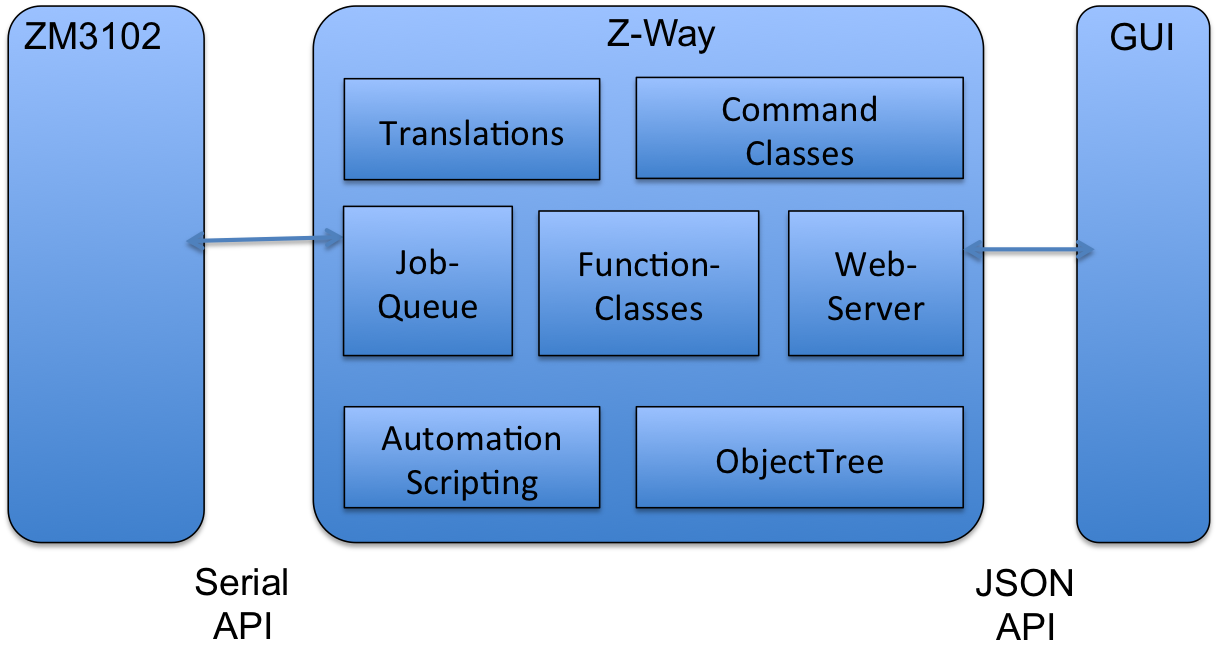
\includegraphics[scale=0.6]{pics/zway1en.png}
\caption{Z-Way Software Structure}
\label{zwaystructure} 
\end{center} 
\end{figure}

Z-Way consists of several function blocks:

\begin{itemize}
\item The Job Queue: This is the core of Z-Way
\item Function Classes: The implementation of all the commands to control the Z-Wave transceiver chip and the Z-Wave network
\item Command Classes: The application level commands used to control Z-Wave devices in the network
\item The JSON web server: It implements the application programmers interface
\item Translation Functions: They help to translate machine readable tokens into human-readable strings
\item The automation and scripting engine: This is the way to get the intelligence into the system.
\end{itemize}

For more information about Z-Way such as the user interface, the JSON API structure etc please refer to the Z-Way User and Developers 
Documentation available online at 
\href{http://razberry.z-wave.me/docs/zway.pdf}{http://razberry.z-wave.me/docs/zway.pdf}


\section{Installation and Start}

{\bf Attention: You must unpower the Raspberry PI board before installing the RaZberry hardware.}
For the installation of the Rasperian OS please refer to the online resources of the Raspberry Pi project. Once the OS is
installed and you are ready to have access to the command line interface of the pertain system, log into the Raspberry Pi with 
the RaZberry hardware attached.

Execute the following command on the command line:
\begin{quote}
{\tt wget -q -O - http://razberry.z-wave.me/install | sudo bash}
\end{quote} 

This script checks if the system is ready to run RaZberry, frees up the serial interface /dev/AMA0 and installs all needed modules. 
After the installation  is complete you can edit the file /opt/Z-Way/config.xml in case you want to change the TCP port the JSON 
web server is running on. After rebooting (unplug/replug power) of the Raspberry Pi open the following page on your web 
browser of choice:
\begin{quote}
{\tt http://IPADDRESSOFRASPBERRY:8083/ }
\end{quote}
or whatever port you have chosen to run the device. If you are already familiar with 
Z-Wave you may want to skip the next section about Z-Wave basics.

 
\end{document} 
